\section{Managementunterstützungssystems}
Hinter dem Begriff Managementunterstützungssystem steckt für alle unter 50 \textit{lobotomized Data Science}, also das Extrahieren von Wissen aus großen Datenmengen, nur ohne Betrachtung der Zukunft und mit einem größeren Fokus auf Berichte von vergangenen Daten.
\begin{figure}[H]
    \centering
    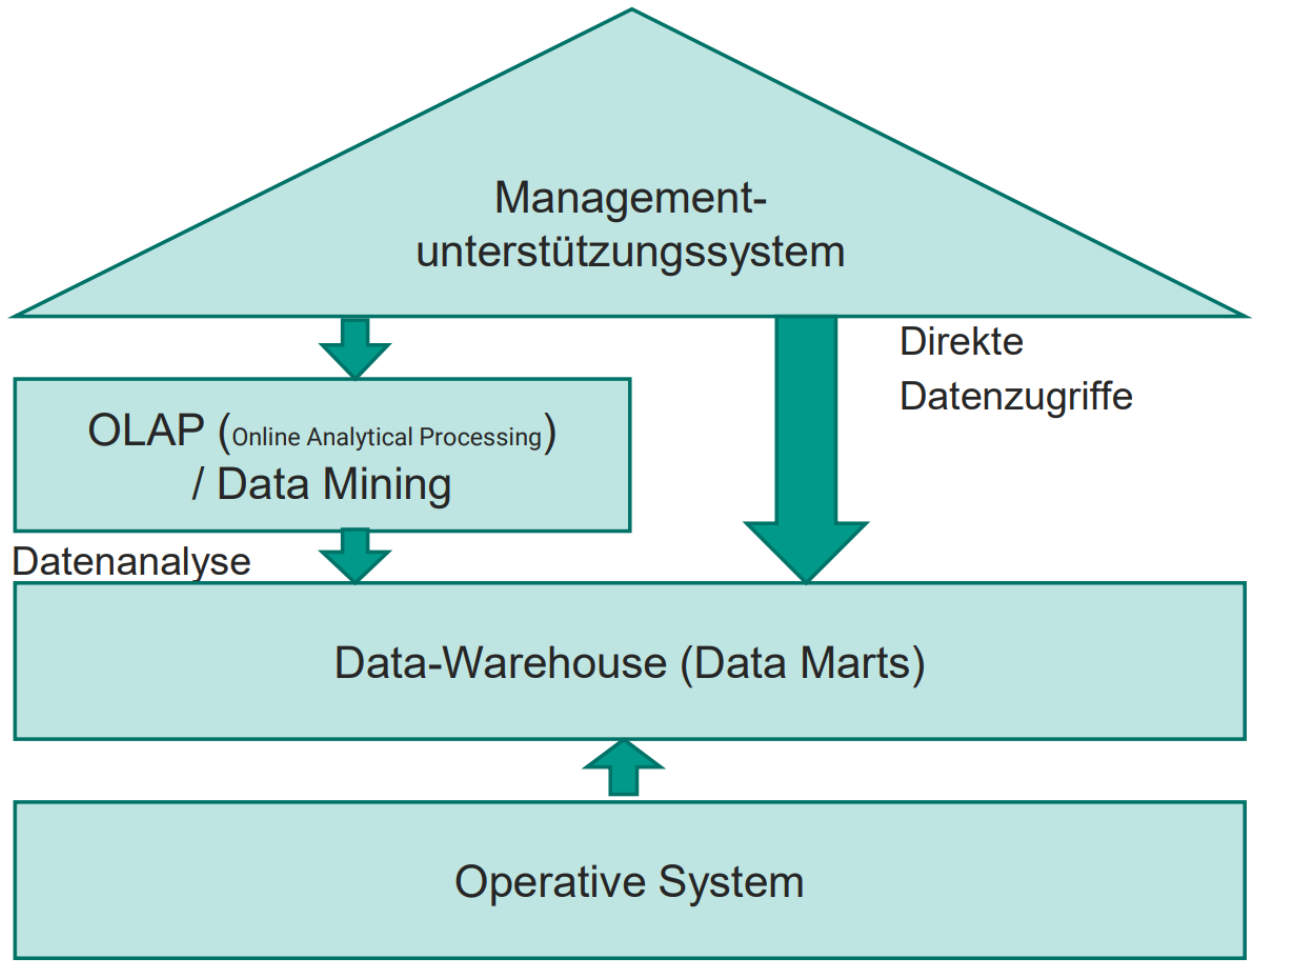
\includegraphics[width=\textwidth]{assets/images/MUS}
    \caption{Aufbau von einem Managementunterstützungssystems}
\end{figure}
\subsection{Data Warehouse}
Data Warehousing beschreibt ein Konzept zur Informations-analyse, -selektion und -aufbereitung, bei dem Anwender entscheidungsrelevante Daten aus unterschiedlichen Quellen in einer einheitlichen zentralen Systemumgebung zur Auswertung zur Verfügung gestellt werden.
\begin{itemize}
    \item Ein Data Warehouse ist eine extrem große Datenbank, die unabhängig von den operativen Systemen installiert ist und ein vordefiniertes Set von meist verdichteten Daten enthält.
    \item Die Benutzer können auf die Datenbank beliebig zugreifen und alle gewünschten Daten herausziehen, sofern die Informationen enthalten sind und eine Zugriffsberechtigung vorliegt.
    \item Der Grad der Informationstiefe und die jeweilige Sichtweise kann dabei individuell festgelegt werden.
    \item Betrachtungsebenen sind beispielsweise Konten, Kostenstellen, Kostenträger, Artikel, Kunden, Märkte oder Vertreter. Es gibt keine festen Vorgaben für die Art der Reihenfolge und der Verdichtung.
\end{itemize}
\subsection{Data Mart}
Data Marts sind abteilungs- oder funktionsbezogene Datenbanken mit einer speziellen Aufgabenstellung,die eine Untermenge der im zentralen Data Warehouse gespeicherten operativen Daten enthalten.
\begin{figure}[H]
  \centering
  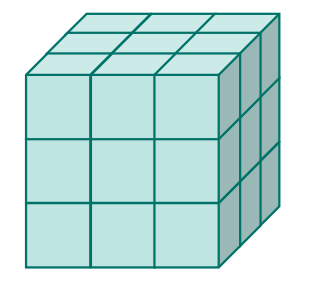
\includegraphics[width=\textwidth]{assets/images/DataMart}
  \caption{Data Mart}
\end{figure}
\begin{itemize}
  \item Data Marts enthalten lediglich Informationen, die in einem bestimmten Funktionsbereich, z.B. Marketing, des Unternehmens zur Anwendung kommen.
  \item Data Marts bilden daher eine Teilmenge der umfassenden Data Warehouse-Datenbank.
  \item Data Marts werden auch Datenwürfel, Power Cube oder Info Cube genannt.
\end{itemize}
\subsection{Online Analytical Processing – OLAP}
Online Analytical Processing ist ein „top-down“-Ansatz, um sehr flexibel mehr dimensionale Daten analysen durchzuführen und Hypothesen zu bilden.
\begin{figure}[H]
  \centering
  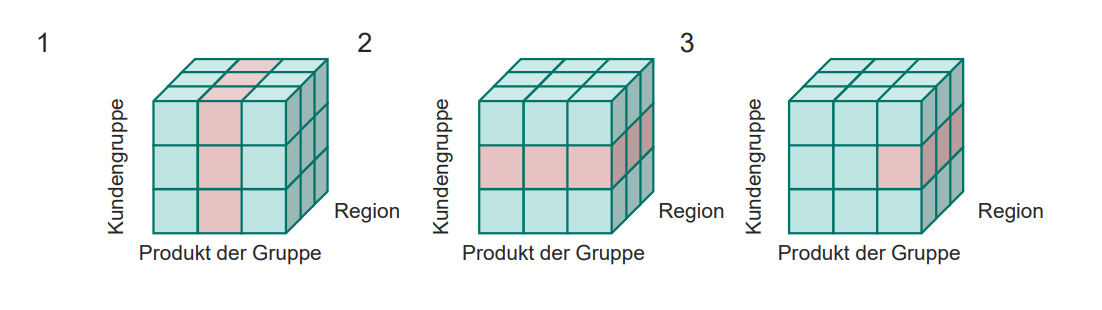
\includegraphics[width=\textwidth]{assets/images/OLAP}
  \caption{Daten Analyse mit OLAP}
\end{figure}
\subsection{Data Mining}
Data Mining bezeichnet das automatische Entdecken von Modellen und Mustern in großen Daten beständen durch Anwendung bestimmter Data Mining-Werkzeuge.
\begin{itemize}
  \item Data Mining ist eine „intelligente“ Anwendung auf Basis einer Data Warehouse-Architektur
  \item Beziehungen zwischen Daten werden hergestellt (Zeitreihenanalyse, Datenklassifikation, Prognosen)
  \item Data Mining versucht den Anwender auf bemerkenswerte Datenkonstellationen aufmerksam zu machen und zu signifikanten Aussagen hinzuführen
  \item Analyseziel: „Finde Gold in Deinen Daten!“
\end{itemize}